\section{A relatív csillapítási tényező szerepe a mozgástörvényben}

\subsection*{Esetek ábrázolása különböző ábrákon}
Az alábbi 4 ábra azonos meglökéses ($v_0 > 0, x_0 = 0$) indítással szemlélteti a $\zeta$ (relatív csillapítási tényező) hatását a rendszer szabadrezgésére.

\begin{figure}[H]
    \centering
    \begin{minipage}{0.48\textwidth}
        \centering
        \textbf{Csillapítatlan ($\zeta = 0$)} \\
        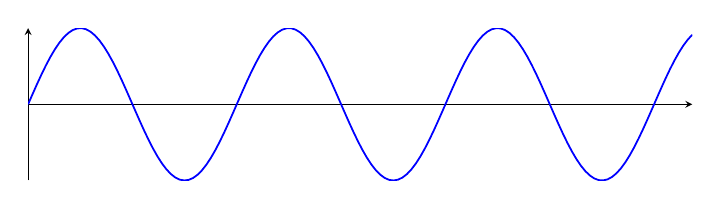
\begin{tikzpicture}[scale=0.8]
            \begin{axis}[axis lines=middle, width=\textwidth, height=4cm, xmin=0, xmax=10, ymin=-1, ymax=1, xtick=\empty, ytick=\empty]
                \addplot[thick, blue, domain=0:10, samples=150] {sin(deg(2*x))};
            \end{axis}
        \end{tikzpicture}
    \end{minipage}\hfill
    \begin{minipage}{0.48\textwidth}
        \centering
        \textbf{Gyengén csillapított ($0 < \zeta < 1$)} \\
        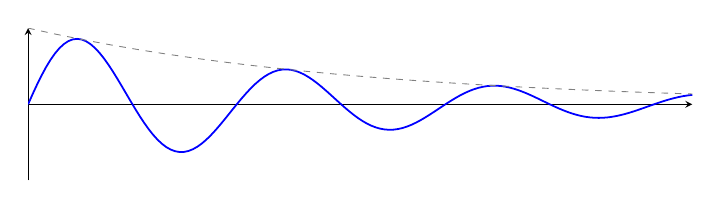
\begin{tikzpicture}[scale=0.8]
            \begin{axis}[axis lines=middle, width=\textwidth, height=4cm, xmin=0, xmax=10, ymin=-1, ymax=1, xtick=\empty, ytick=\empty]
                \addplot[thick, blue, domain=0:10, samples=150] {exp(-0.2*x)*sin(deg(2*x))};
                \addplot[dashed, gray, domain=0:10] {exp(-0.2*x)};
            \end{axis}
        \end{tikzpicture}
    \end{minipage}
    
    \vspace{0.5cm}
    \begin{minipage}{0.48\textwidth}
        \centering
        \textbf{Kritikusan csillapított ($\zeta = 1$)} \\
        \begin{tikzpicture}[scale=0.8]
            \begin{axis}[axis lines=middle, width=\textwidth, height=4cm, xmin=0, xmax=10, ymin=-0.2, ymax=1, xtick=\empty, ytick=\empty]
                \addplot[thick, blue, domain=0:10, samples=150] {2*x*exp(-2*x)};
            \end{axis}
        \end{tikzpicture}
    \end{minipage}\hfill
    \begin{minipage}{0.48\textwidth}
        \centering
        \textbf{Erősen csillapított ($\zeta > 1$)} \\
        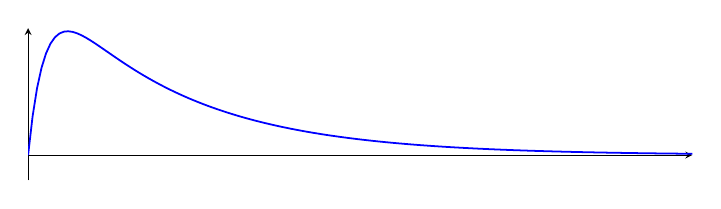
\begin{tikzpicture}[scale=0.8]
            \begin{axis}[axis lines=middle, width=\textwidth, height=4cm, xmin=0, xmax=10, ymin=-0.2, ymax=1, xtick=\empty, ytick=\empty]
                \addplot[thick, blue, domain=0:10, samples=150] {1.5*(exp(-0.5*x) - exp(-4*x))};
            \end{axis}
        \end{tikzpicture}
    \end{minipage}
    \caption{A mozgástörvények alakjai különböző relatív csillapítási tényezők mellett.}
\end{figure}

\subsection*{A periódusidő és a csillapodás ütemének változása}
Ahogy a csillapítás ($\zeta$) növekszik:
\begin{itemize}
    \item \textbf{Csillapodás üteme:} Egyre gyorsabban emészti fel a rendszer a kezdeti mozgási energiát, a burkológörbe negatív exponenciális kitevője egyre markánsabb ($e^{-\zeta\omega_n t}$), így a lengések hamarabb halnak el.
    \item \textbf{Periódusidő változása:} Ezzel egyidőben a rezgés lelassul. A csillapított sajátkörfrekvencia $\omega_d = \omega_n \sqrt{1-\zeta^2}$ csökken, ami a $T_d = \frac{2\pi}{\omega_d}$ kvázi-periódusidő megnövekedését jelenti a csillapítatlan $\zeta=0$ esethez képest. Így a lengések ritkábbak és elnyújtottabbak lesznek. Amikor $\zeta \ge 1$ (kritikus és felette), már nem értelmezünk periódusidőt, mivel a lengés nyomtalanul eltűnik, aperiodicussá válik a mozgás.
\end{itemize}

\subsection*{Miért kiemelt a kritikus csillapítás?}
A kritikus csillapítás ($\zeta = 1$) \textbf{kiemelt jelentőségű a mérnöki gyakorlatban}, mert ez felel meg a lengések nélküli, legrövidebb idő alatti egyensúlyba való beállás ("nyugalomba térés") elméleti határának. Minden más $\zeta > 1$ (erősen csillapított) esetben a tömeg, bár nem lendül át a túlsó oldalra, a megnövekedett fékezőerő miatt túl lomhán, lassabban simul rá az aszimptotikus nulla állapotra. Ha minél rövidebb idő alatt, túllendülés nélkül akarunk megállítani egy rendszert (pl. löveg hátrasiklása méréseknél, mutatós műszerek lecsillapítása, járművek lengéscsillapítóinak optimalizálása), akkor az elméleti optimum a $\zeta=1$ beállítása.
